\chapter{Progettazione e codifica}

\section{Tecnologie utilizzate}

\subsection{Vue}
\begin{figure}[H]
	\begin{center}
		
\includegraphics[width=0.7\columnwidth]{immagini/vue.png}
		\caption{Logo di Vue.js}
	\end{center}
\end{figure}
Vue.js è un framework javascript open source nato nel 2013 che presenta un'architettura adottabile in modo incrementale che si concentra sulla composizione dei componenti, inoltre sono presenti funzionalità avanzate offerte tramite librerie e pacchetti di supporto. I componenti Vue estendono gli elementi HTML di base per incapsulare del codice riutilizzabile quindi a livello generale i componenti sono elementi personalizzati a cui il compilatore Vue associa una particolare funzionalità.\\
Vue utilizza quindi una sintassi basata su HTML e consente di associare il DOM renderizzato ai dati dell'istanza di Vue sottostante. In questo modo i modelli Vue possono essere analizzati da browser e parser HTML conformi alle modifiche ed inoltre con il sistema di reattività Vue è in grado di calcolare il numero minimo di componenti per eseguire nuovamente il rendering applicando la quantità minima di manipolazioni DOM quando cambia lo stato dell'app. Vue presenta un sistema reattivo grazie all'utilizzo di oggetti semplici Javascript ed ad un re-rendering ottimizzato: ogni componente durante il render tiene traccia delle sue dipendenze in modo tale che il sistema sappia quando e di quali componenti deve effettuare nuovamente il render.\\
Un problema che afflige le web application a pagina singola è che quest'ultime forniscono agli utenti la risposta basata solamente sull'URL dal server, di conseguenza l'utilizzo dei segnalibri a determinate schermate e la condivisione dei collegamenti a sezioni specifiche risulta molto difficile se non impossibile. Vue.js per riuscire a risolvere questo problema fornisce un'interfaccia, detta router, che da la possibilità di modificare ciò che viene visualizzato sulla pagina in base all'URL indipendentemente da come esso viene modificato. Infatti Vue.js viene fornito con il pacchetto open source "vue-router" che fornisce un'API per aggiornare l'URL dell'applicazione, supportare la cronologia di navigazione e le reimpostazioni di email e password. Tramite questa tipologia di router i componenti devono essere mappati alla route a cui appartengono per indicare dove deve essere eseguito il loro render.\\
Questo framework implementa il pattern MVVM, acronimo per Model-View-View-Model, una declinazione del più famoso MVC, ovvero Model-View-Controller. I componenti del MVVM sono:
\begin{itemize}
	\item Model (o Modello): l'implementazione del dominio dati come per il classico Modello del pattern MVC;
	\item View (o Vista): il componente grafico renderizzato dall'utente formato da HTML e CSS;
	\item ViewModel (o Vista per il Modello): il collante tra gli altri due componenti, esso fornisce alla View i dati in formato consono alla rappresentazione ed il comportamento di alcuni elementi dinamici.
\end{itemize}
La grossa differenza tra il pattern implementato da Vue.js e il Model-View-Controller sta nella differenza tra Controller e ViewModel. Il primo, infatti, è una porzione di codice che gestisce la logica di business grazie al Model e ritorna una View da mostrare all'utente; il secondo, invece, rappresenta una versione parallela al Model che risulta essere legato alla View e descrive il comportamento di quest'ultima con funzioni associate. Quindi mentre il Controller esegue logiche di business prima del rendering della View, il ViewModel definisce il comportamento dell'applicazione a runtime.

\subsection{Vuetify}
Vuetify è un framework UI completo costruito su Vue.js nel 2014 ed il suo obiettivo è fornire agli sviluppatori gli strumenti per poter creare esperienze utente ricche e coinvolgenti. A differenza di altri framework Vuetify è progettato da zero in modo tale da renderlo facile da imparare ed essere gratificante da padroneggiare con centinaia di componenti realizzate dalle specifiche di Material Design.\\
Un pregio di questo framework è che adotta un approccio al mobile, questo significa che la web application sviluppata tramite esso sarà pienamente utilizzabile immediatamente su un tablet, un telefono ed un computer. Inoltre è un framework in sviluppo attivo che viene aggiornato settimanalmente rispondendo ai problemi e relativi report della community. Un altro pregio è, come si può vedere nell'immagine sottostante, il gran numero di funzionalità che possiede Vuetify in confronto agli altri framework di Vue.
\begin{figure}[H]
	\begin{center}
		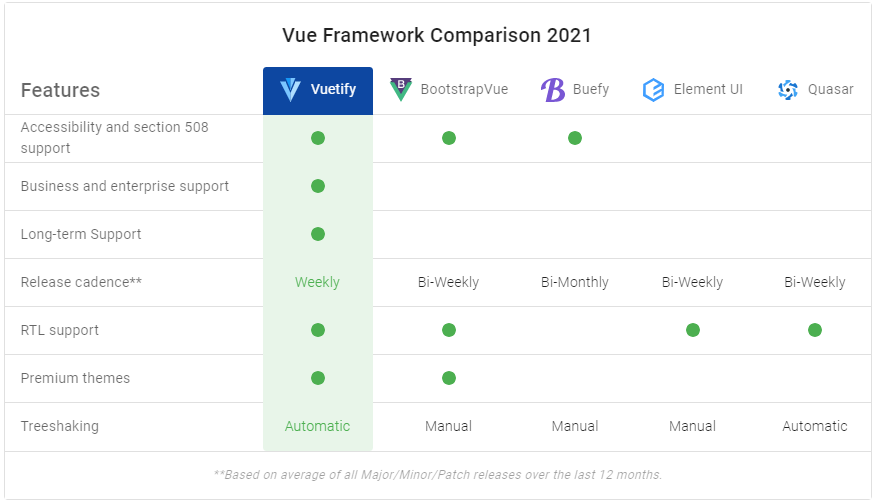
\includegraphics[width=1\columnwidth]{immagini/vuetify.png}
		\caption{Funzionalità di Vuetify}
	\end{center}
\end{figure}
\subsection{Vuex}
Vuex è uno state management pattern per applicazioni sviluppate in Vue.js e serve come store centralizzato per tutti i componenti dell'applicazione. Esso contiene stati e regole che assicurano che lo stato può essere modificato solo in modo prevedibile.

\section{Organizzazione dei file}
Quando si crea un progetto per la prima volta tramite il framework Vue.js vengono create di default delle cartelle e dei file per facilitare la progettazione del software. La suddivisione delle cartelle è rappresentata qui di seguito.

\begin{lstlisting}
	|-- front-end-vue
	|-- .editorconfig
	|-- .eslintignore
	|-- .eslintrc.js
	|-- .gitignore
	|-- .prettierc.json
	|-- .prettierignore
	|-- babel.config.js
	|-- jest.config.js
	|-- jsconfig.json
	|-- package-lock.json
	|-- package.json
	|-- README.md
	|-- vue.config.js
	|-- .vscode
	| |-- extensions.json
	| |-- settings.json
	|-- coverage
	|-- dist
	|-- docs
	|-- pubblic
	|-- src
	| |-- App.vue
	| |-- directoryList.md
	| |-- main.js
	| |-- assets
	| |-- components
	| |-- plugins
	| |-- router
	| |-- store
	| | |-- index.js
	| | |-- modules
	| | |-- currentUser.js
	| | |-- nftService.js
	| |-- view
	|-- tests
	| | |-- unit
\end{lstlisting}

La cartella principale si chiama \textbf{\textit{front-end-vue}} ed essa contiene i file di configurazione del progetto, il file \textbf{\textit{readme}} ed il file di \textbf{\textit{gitignore}}. I file e le sottocartelle create automaticamente alla creazione del progetto non verranno spiegate, mentre i restanti elementi sono i seguenti:
\begin{itemize}
	\item \textbf{\textit{coverage}}: cartella che contiene i file e le cartelle create automaticamente quando vengono fatti partire i test di unità;
	\item \textbf{\textit{doc}}: cartella che contiene file YAML utilizzato per la configurazione di Stoplight;
	\item \textbf{\textit{src}}: cartella in cui sono presenti file e cartelle necessari per il funzionamento del progetto e sono:
	\begin{itemize}
		\item il file \textbf{\textit{App.vue}} è la radice dell'applicazione definita nel formato Vue Component e di solito serve a definire il modello della pagina;
		\item il file \textbf{\textit{directoryList.md}} che viene creato automaticamente attraverso il comando \textit{mddir} dove viene scritta la struttura delle cartelle del progetto;
		\item il file \textbf{\textit{Main.js}} di tipo javascript che inizializza il file \textit{App.vue} ed è responsabile dell'impostazione dei plugin e dei componenti di terze parti da utilizzare per lo sviluppo dell'applicazione;
		\item la cartella \textbf{\textit{assets}} contenente le immagini utilizzate all'interno del sito, come quella del logo;
		\item la cartella \textbf{\textit{components}} contenente la barra di navigazione (navbar) e le varie finestre d'avviso;
		\item la cartella \textbf{\textit{plugins}} contenente i file javascript dei plugin utilizzati per lo sviluppo, in questo caso di Vuetify;
		\item la cartella \textbf{\textit{router}} contenente un omonimo file javascript dove vengono definite le route ovvero le varie pagine in cui può navigare l'utente;
		\item la cartella \textbf{\textit{store}} contenente i file per la configurazione delle chiamate al database e lo state management;
		\item la cartella \textbf{\textit{view}} contenente le possibili schermate che può visualizzare l'utente;
		\item la cartella \textbf{\textit{tests}} che contiene la sottocartella \textbf{\textit{unit}} dove sono presenti i test di unità effettuati.
	\end{itemize}
\end{itemize}

\textit{Nelle sezioni di seguito verranno spiegate in dettaglio il funzionamento delle chiamate al back end e delle varie maschere implementate con le loro criticità}

\section{Chiamate al back end}
Il file principale, \textbf{\textit{index.js}}, contiene la configurazione di Vuex e del persisted state con l'inclusione dei moduli tanti quanti sono i servizi del back end che vanno ad invocare. (NON MI PIACE) Per rendere più chiaro ed efficiente il lavoro ho creato tanti file quanti sono i servizi che vado ad invocare quindi sono presenti il file \textbf{\textit{CurrentUser.js}}, legato al servizio del back end dell'utente, e il file \textbf{\textit{NftService.js}}, legato al servizio del back end degli NFT.\\
Entrambi i file hanno la struttura uguale e quello che cambia è il contenuto, infatti sono caratterizzati da tot variabili costanti:
\begin{itemize}
	\item state, contenente le risorse che verranno utilizzate nei metodi;
	\item actions, contenente i metodi dove vengono fatte le invocazioni ai servizi del backend tramite axios;
	\item mutations, contenente i metodi che modificano le risorse, sono come un equivalente dei metodi set;
	\item getters, contenente i metodi che ritornano i valori presenti nelle risorse.
\end{itemize}

Gli state del file \textbf{\textit{CurrentUser.js}} li ho resi persistenti, in questo modo potranno essere utilizzati all'interno della web application. Ad esempio nel momento in cui l'utente effettua il login la variabile booleana \textit{loggedIn} viene settata a \textit{true} e può essere utilizzata per fare dei controlli che decidono(VERBO MIGLIORE?) se reindirizzare o meno certe parti della web application.\\
Essendo legati a servizi diversi i metodi e le chiamate al back end dei due file sono molto diversi; infatti ad esempio nel file \textbf{\textit{CurrentUser.js}} ho implementato il metodo \textit{loginUser} che effettua una POST per autenticare l'utente nel sito salvando le sue informazioni per poterle utilizzare dove necessario, mentre nel file \textbf{\textit{NftService.js}} ho implementato il metodo \textit{uploadOpera} che effettua una POST per salvare una nuova opera nel database.

\section{Maschere implementate}

Per comprendere meglio il funzionamento delle maschere queste verranno spiegate suddivise in base alla cartella di appartenenza, ovvero la cartella \textbf{\textit{View}} e la cartella \textbf{\textit{Components}} (NON mi piace)

\subsection{View}
\subsubsection{Home}
Pagina principale del sito tramite la quale l'utente può visualizzare tutte le opere presenti in esso e, selezionata una di queste, potrà visualizzare nel dettaglio tutte le sue informazioni. Una parte importante è la presenza di una barra di navigazione che aiuta l'utente a navigare all'interno del sito.
\subsection{Login}
In questa pagina l'utente può effettuare l'autenticazione nel sito tramite email e password. In questi due campi sono state inserite delle regole che, se non rispettate, generano un errore visualizzabile tramite una scritta sotto il campo che si sta modificando. Le regole in questione sono:
\begin{itemize}
	\item entrambi i campi sono obbligatori, quindi devono essere tutti compilati;
	\item l'email inserita deve essere valida\\
	\textit{esempio di email valida: nome@email.it};
	\item la password deve avere una lunghezza di minimo otto caratteri di cui almeno una lettera maiuscola, una minuscola, un numero e una carattere speciale.
\end{itemize}
\subsection{Registrazione}
In questa pagine l'utente può effettuare la registrazione nel sito inserendo: nome, cognome, email, data di nascita, wallet address, password e conferma password. Similmente alla pagina di login sono state inserite delle regole che, se non rispettate, generano un errore visualizzabile tramite una scritta sotto il campo che si sta modificando. Le regole in questione sono:
\begin{itemize}
	\item tutti i campi sono obbligatori, quindi devono essere tutti compilati;
	\item l'email inserita deve essere valida\\
	\textit{esempio di email valida: nome@email.it};
	\item la data di nascita deve corrispondere ad una persona maggiorenne;
	\item il wallett address inserito deve essere valido\\ 
	\textit{esempio di wallett address valido: 0x390c7a1EA64e521B725b1869Ea054DDBF05F9abe};
	\item la password deve avere una lunghezza di minimo otto caratteri di cui almeno una lettera maiuscola, una minuscola, un numero e una carattere speciale;
	\item la conferma della password deve essere identica alla password appena inserita.
\end{itemize}
\subsection{Pagina dell'utente}
In questa pagina l'utente può visualizzare le sue informazioni personali e le opere che possiede. Nel momento che verranno modificate le informazioni tramite le funzioni apposite da parte dell'utente, queste verranno modificate a schermo automaticamente.
\subsubsection{Upload opera}
In questa pagina è possibile per l'utente aggiungere una nuova opera. I campi da compilare sono: titolo, descrizione, file, prezzo. Quando l'utente carica un file verranno generati automaticamente una preview del file specifica in base al tipo del file inserito e un campo non modificabile che indica il tipo del file inserito. Similmente alla pagina di registrazione sono state inserite delle regole che, se non rispettate, generano un errore visualizzabile tramite una scritta sotto il campo che si sta modificando. Le regole in questione sono:
\begin{itemize}
	\item tutti i campi sono obbligatori, quindi devono essere tutti compilati.
\end{itemize}
\subsection{Components}
\subsubsection{Barra di navigazione}
Questa componente è presente in quasi tutto il sito ad eccezione delle pagine di Login e di Registrazione. Per poter implementare questo dettaglio il componente che ha il compito di reindirizzarla, ovvero il file \textbf{\textit{App.vue}}, possiede una condizione dove viene fatto il controllo se la pagina in cui si sta navigando sia una di quelle dove deve essere presente o meno la Navbar. Se il controllo va a buon fine la Navbar verrà reindirizzata, altrimenti non verrà mostrata all'utente.\\
Un'altra particolarità di questo componente è la presenza di due bottoni che variano in funzione se l'utente è autenticato o meno nel sito. Infatti se l'utente non si autentica si vedranno due bottoni per effettuare il login o la registrazione, mentre se esso è autenticato si bottoni serviranno per visualizzare la pagina personale oppure effettuare il logout. Per gestire questa particolarità è stato implementato un if else (HA UN NOME QUESTA COSA) dove controlla appunto lo stato dell'utente tramite una variabile chiamata \textit{isLogged}, vera se autenticato.
\subsubsection{Gestione opere}
L'utente può unicamente modificare una sua opera ma non può cancellarla. Questo è dovuto al fatto che al momento dell'upload l'opera verrà caricata sulla blockchain rendendola un elemento unico ed irripetibile quindi non può cancellarla. Per motivi analoghi l'utente ha delle restrizioni anche nella modifica dell'opera; infatti di essa può modificare solo: titolo, descrizione, prezzo e categorie di appartenenza. Un altro campo non modificabile è il tipo del file caricato.
\subsubsection{Modifica dati personali}
L'utente, dopo aver premuto un bottone con la dicitura "Modifica dati personali", vedrà apparire una finestra di avviso dove può modificare i propri dati. Per motivi di univocità l'utente non potrà modificare l'email con cui ha fatto l'accesso, infatti potrà modificare solamente il nome ed il cognome. Inoltre per motivi di sicurezza il bottone per confermare la modifica è disabilitato di default e viene data la possibilità di confermare la modifica solo dopo aver inserito la password corrente.
\subsubsection{Modifica password}
L'utente dopo aver premuto un bottone con la dicitura "Modifica password", vedrà apparire una finestra di avviso dove può modificare la password. Per poterlo fare, per motivi di sicurezza, l'utente dovrà inserire la sua email, la password corrente e la nuova password. Similmente alla modifica dei dati personali, il bottone per confermare la modifica rimarrà disattivato fino a quando l'utente non avrà completato tutti i campi.